\documentclass[letterpaper,11pt]{article}
\oddsidemargin -1.0cm \textwidth 17.5cm

\usepackage[utf8]{inputenc}
\usepackage[activeacute,spanish]{babel}
\usepackage{amsfonts,setspace}
\usepackage{amsmath}
\usepackage{amssymb, amsmath, amsthm}
\usepackage{comment}
\usepackage{amssymb}
\usepackage{dsfont}
\usepackage{anysize}
\usepackage{multicol}
\usepackage{enumerate}
\usepackage{graphicx}
\usepackage[left=1.5cm,top=2cm,right=1.5cm, bottom=1.7cm]{geometry}
\setlength\headheight{1.5em} 
\usepackage{fancyhdr}
\usepackage{multicol}
\usepackage{hyperref}
\usepackage{wrapfig}
\usepackage{subcaption}
\pagestyle{fancy}
\fancyhf{}
\renewcommand{\labelenumi}{\normalsize\bfseries P\arabic{enumi}.}
\renewcommand{\labelenumii}{\normalsize\bfseries (\alph{enumii})}
\renewcommand{\labelenumiii}{\normalsize\bfseries \roman{enumiii})}

\begin{document}

\fancyhead[L]{\itshape{Facultad de Ciencias F\'isicas y Matem\'aticas}}
\fancyhead[R]{\itshape{Universidad de Chile}}

\begin{minipage}{11.5cm}
    \begin{flushleft}
        \hspace*{-0.6cm}\textbf{FI1000-1 Introducción a la Física Clásica}\\
        \hspace*{-0.6cm}\textbf{Profesora:} Paulina Lira\\
        \hspace*{-0.6cm}\textbf{Auxiliares:} Alejandro Silva, Juan Cristóbal Castro\\
    \end{flushleft}
\end{minipage}

\begin{picture}(2,3)
    \put(366,-4){
\includegraphics[scale=0.9]{2020-1/Imágenes/logo/dfi-fcfm.pdf}}
\end{picture}

\begin{center}
	\LARGE \bf Auxiliar \# 10\\
\end{center}

\vspace{-1cm}
\begin{enumerate}\setlength{\itemsep}{0.4cm}

\rfoot[]{pág. \thepage}

\item[]

\item Una partícula colisiona a una segunda partícula de igual masa que estaba inicialmente en reposo. Si colisionan elásticamente sobre un plano horizontal libre de roce, determine el ángulo $\phi$ de salida de la partícula inicialmente en reposo si la primera partícula se desvía un ángulo $\theta$ con respecto a la dirección que traía antes de la colisión.

\begin{figure}[h!]
    \centering
    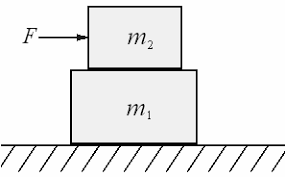
\includegraphics[scale=0.5]{2020-1/Imágenes/aux13/images.png}
\end{figure}

\item Sobre una plataforma horizontal sin roce se colocan en línea recta 99 bloques separados entre sí una cierta distancia, en donde el $n$-ésimo bloque tiene masa $(n+1) m$. Desde la izquierda incide un bloque de masa $m$ con velocidad $v_0$. Todos los choques son perfectamente elásticos.
    \begin{enumerate}
        \item Calcule la velocidad del bloque de masa $2m$ inmediatamente después de la primera colisión.
        \item Calcule la velocidad del bloque de masa $2m$ inmediatamente después que experimenta el segundo choque.
        \item Después de un tiempo suficientemente largo se observa que ningún bloque permanece sobre la plataforma. ¿Cuántos bloques cayeron al lado izquierdo y cuántos al lado derecho?
    \end{enumerate}

\begin{figure}[h!]
    \centering
    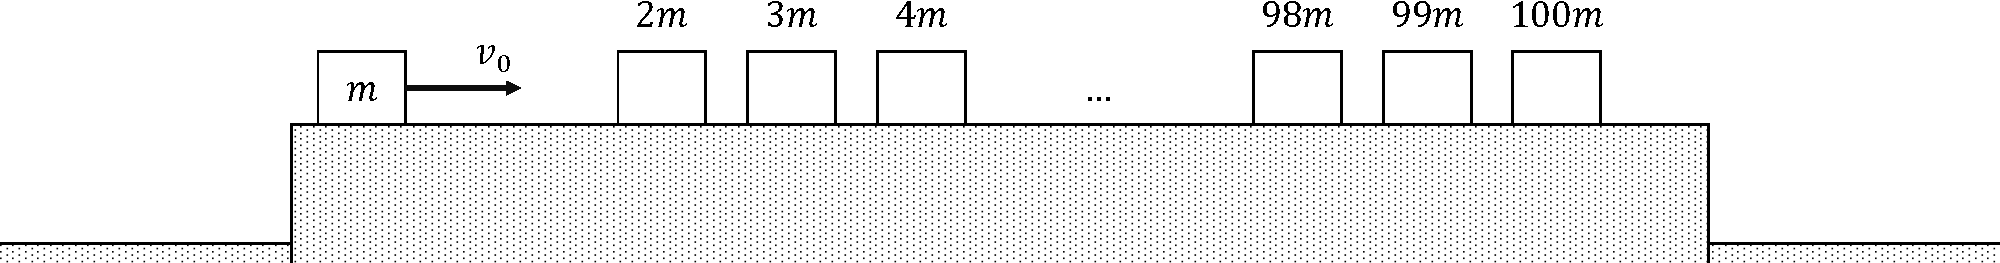
\includegraphics[scale=0.35]{2020-1/Imágenes/aux13/100masas.pdf}
\end{figure}


\item Una masa $m$ es soltada desde el punto más alto de un tazón semiesférico de radio $R$, encontrándose en su camino con otra masa de las mismas características, la cual está en reposo en el punto más bajo de aquel, quedando unidas tras el impacto. 
\begin{enumerate}
    \item Despreciando la fricción entre las masas y el tazón, determine la altura máxima alcanzada por el sistema. 
    \item Compare la energía de la situación inicial y final.
    
    \begin{figure}[h!]
    \centering
        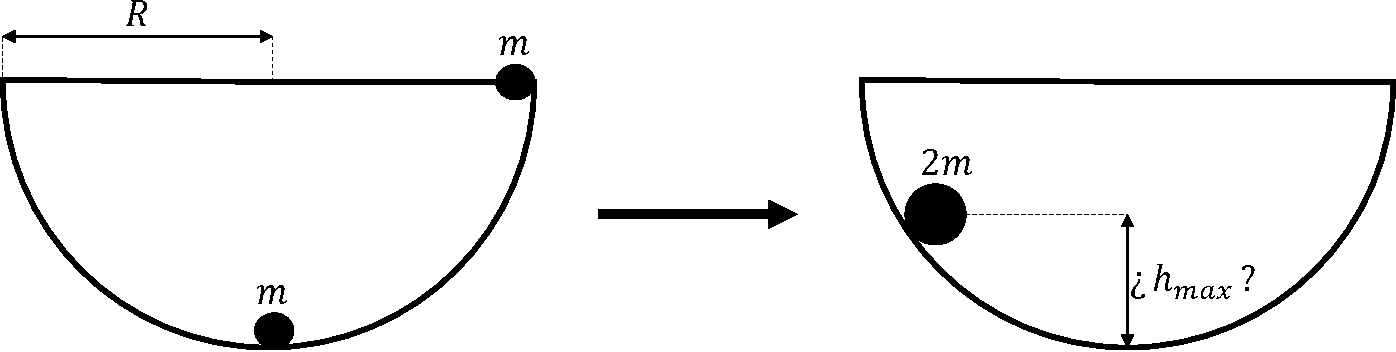
\includegraphics[scale=0.3]{2020-1/Imágenes/aux13/sem.pdf}
        \caption*{Figura P3}

\end{figure}
\end{enumerate}

\end{enumerate}
\end{document}